\section{Investigation into effects of ODB complexity (V-2)}
\label{sect:exp_complexity}

\subsection{Introduction}
Phase 2 models, whether real ODB snapshots or generated are likely to vary somewhat in the range of characteristics measured by the various complexity metrics (PCMs). 

The main aims of this investigation are to determine the similarities and differences between real and generated models, the range of variation between generated models created using the same parameters sets and to determine if different schedulers perform better than others when faced with Phase 2 models with different \emph{weight} or \emph{loading} characteristics. It is hoped to be able to answer questions such as whether one scheduler is better at handling \emph{light} loading and perhaps a different scheduler is better at handling \emph{heavy} loading.

\subsection{Choice of PCM to characterise a Phase 2 model} 
We have seen from Sect.~\ref{sect:metrics} that there are several complexity metrics (PCMs) available. None of these are able to fully characterize the loading as this varies through the night and from day to day and is dependant on what has (or might have) occurred previously. Of the serveral contenders, the average contention $C_C$ was chosen. This is a metric which is easy to calculate and readily visualized.
 
\subsection{Comparison of real and generated Phase 2 models} 
A Phase2 model generator (P2GEN) was designed to create Phase 2 models with varying characteristics. This generator, described in Appendix (XX) has a large number of configurable parameters. The main parameters in terms of the current study however are the number of proposals, groups per proposal, observations per group and mean exposure time. The latter determine the length of each group, the others how many groups are in the \emph{pool}. Table.~\ref{tab:ltc_p2models} summarizes the model and snapshot parameters.

\begin{table}[h]
 \begin{center}
  \begin{tabular}{lllll}
   \toprule
   \multicolumn{5}{c}{Phase2 models - more detail required} \\
   \midrule
   DBID & ODB Date & $N_p$ & $N_g$ & Description\\
   \midrule
   $P_s$ & 22/11/07 midpoint & 10 & 10 & P2GEN small model \\
   $P_l$ & 22/11/07 midpoint & 15 & 20 & P2GEN light model \\
   $P_m$ & 22/11/07 midpoint & 30 & 30 & P2GEN medium model\\
   $P_h$ & 22/11/07 midpoint & 50 & 50 & P2GEN heavy model \\
   \midrule
   $O_1$ & 15/10/07 snapshot & - & - & ODB snapshot Day 0\\
   $O_2$ & 25/09/07 snapshot & - & - & ODB snapshot Day -20\\
   \bottomrule
  \end{tabular}
 \end{center}
\caption{Phase2 model descriptions - need more info on these than what is in table esp the gen models}
\label{tab:ltc_p2models}
\end{table}


A set of simulations were performed over a period of 60 days for each of the 4 generated models $P_l$ - $P_h$ to guage the level of contention these would yield and to compare with sample ODB snapshots for the same period. The results of a single simulation run for each model are shown in figures \ref{fig:c60_gen_av} and \ref{fig:c60_gen_ng}. Similar figures for the ODB snapshots are shown in \ref{fig:c60_odb_av} and \ref{fig:c60_odb_ng}.

\begin{figure}[h]
\begin{center}
 \subfigure[Variation of average contention $\bar{C_c}$ for generated phase2 models.] {
   \includegraphics[scale=0.5, angle=-90]{figures/c60_gen_cav.eps}  
   \label{fig:c60_gen_av}
  }
 \subfigure[Variation of number of executed groups for generated phase2 models.] {
   \includegraphics[scale=0.5, angle=-90]{figures/c60_gen_ng.eps}  
   \label{fig:c60_gen_ng}
  }
  \caption{Comparison of average contention measure and number of groups executed per night for generated Phase 2 models.}
 \end{center}
\end{figure}

\begin{figure}[h]
\begin{center}
 \subfigure[Variation of average contention $\bar{C_c}$ for ODB snapshots.] {
   \includegraphics[scale=0.5, angle=-90]{figures/c60_odb_cav.eps} 
   \label{fig:c60_odb_av}
  }
 \subfigure[Variation of number of executed groups for ODB snapshots.] {
   \includegraphics[scale=0.5, angle=-90]{figures/c60_odb_ng.eps}  
   \label{fig:c60_odb_ng}
  }
  \caption{Comparison of average contention measure and number of groups executed per night for ODB snapshots.}
 \end{center}
\end{figure}

%% Analysis
In addition to variation in characteristics, the real Phase 2 models suffer from a population evolution problem. From  Fig.~\ref{fig:c60_odb_av} which shows the variation of average nightly contention $C_C$ for ODB snapshots taken on the first night of the 60 day period ($O_1$) and on a night 20 days before the start of the same period ($O_2$), we see the overall contention seems to decline over the period. We also note in particular that the contention figures for $O_2$ are generally lower than for snapshot $O_1$. These effects are infact due to the pattern in which observations are entered into the system. A sizeable number of observations are \emph{short-term} and only entered into the ODB a day or so before they are required. In some cases, particularly where automated agents are involved, the observations may be entered minutes before they become activated. This information cannot be captured by a snapshot of the ODB at a given time and so the observed quality and characterisation measures drift away from what would be observed if the ODB model were being regularly replenished.

With a generated model however, groups can all be entered at the start but with their activations spread out over a specified period (say several months) so new groups are appearing in the schedule every day. The day to day loading as shown in Fig.~\ref{fig:c60_gen_av} appears to remain more constant like that of a real ODB if we were to take daily snapshots. 


\subsection{Characterisation of generated models}
\label{sect:chargen}
 From a given generator model (e.g. $P_l$) we can generate any number of actual instances. Ideally these would all have the same measurable characteristics (e.g. $\bar{C_c}$) but this is not guaranteed. Further, it is not possible with P2GEN to easily generate a specific Phase 2 model instance with a specific set of PCM characteristics.

Consequently in order to explore the range of these characteristics it is neccessary to generate a number of different models from the same generator parameters and then measure the characteristic of these models either by simulation to obtain dynamic measures or by a straightforward measurement of the static characteristics.

A set of 4 model generators were chosen and are described in more detail in Table.~\ref{tab:ltc_p2models}. These generators are selected to represent a range of characteristics from \emph{small}, designed to create low-load Phase 2 models upto \emph{heavy}, designed to generate high load models. Tests were performed on 25-30 models generated by each generator to allow these to be characterised in terms of the chosen PCM, average contention ($C_C$). A series of simulations were then performed on each model to generate a set of SQMs, specifically $Q_{SU}$ - a score based metric and $Q_{XT}$ - the fraction of night observed. 

The measurable characteristic chosen was $\bar{C_{dc}}$ - the average dynamic contention over the measurement period. A simple scheduler was chosen using best-score selection and a single $f_{OH}$ metric - i.e. the target which was highest relative to maximum attainable elevation was chosen at each sweep. In these simulations we are not particularly interested in the scheduler here, only in the variability of the generated  Phase 2 characteristics. Simulations were run for the middle 30 days of the generated models and the values of $\bar{Q_{SU}}$ and $\bar{Q_{XT}}$ are plotted against $\bar{C_c}$ for each model. The results are shown in Fig.~\ref{fig:p2_gen_su} and  Fig.~\ref{fig:p2_gen_xt}.



\begin{figure}[h]
\begin{center}
 \includegraphics[scale=0.5, angle=-90]{figures/p2_gen_qsu.eps}
 \caption[Variation of $Q_{SU}$ with $C_{DC}$ for variable phase2 generator models.] 
   {Variation of $Q_{SU}$ with $C_{DC}$. Each point represents a single phase 2 model generated by one of 4 initial sets of generators.}
\label{fig:p2_gen_su}
\end{center}
\end{figure}


\begin{figure}[h]

\begin{center}
 \includegraphics[scale=0.5, angle=-90]{figures/p2_gen_qxt.eps}
 \caption[Variation of $Q_{XT}$ with $C_{DC}$ for variable phase2 generator models.] 
   {Variation of $Q_{XT}$ with $C_{DC}$. Each point represents a single Phase 2 model generated by one of 4 initial sets of generators.}
\label{fig:p2_gen_xt}
\end{center} 
\end{figure}

From these results it is clear there is significant variation in the measurable characteristics for any model though there is a progression between models as might be expected i.e. most of the $P_l$ contention values are lower than most of the $P_h$ values. There is significant overlap between \emph{adjacent} models. The heavy model generally uses up all or very nearly all of the available night. This is not too surprising, there are more groups to chose from so there are likely to be few if any slack periods. There is most variation in $Q_{SU}$ for the small and light models, with low contention there will be periods when no groups are actually schedulable hence the frequent depression of this metric and in the overall use of time.

\subsection{Comparison of schedulers against variable loading characteristics}
In order to establish the effectiveness of different schedulers against ODB loading a number of simulations were performed. The BDS scheduler was tested using the \emph{best}, \emph{rank score biased} and \emph{fixed rank biased} selection models. QLAS was tested using horizons of 1,2 and 4 hours. Details of biased selection models are to be found in Sect.~\ref{sect:ss_exptsetup}.

\begin{figure}[h]
 
\begin{center}
 \includegraphics[scale=0.5, angle=-90]{figures/qsucc_best.eps}
 \caption[Effect of selection model on variation of $Q_{SU}$ with $C_c$ for BDS using $\zeta_{Best}$.] 
   {Effect of selection model on variation of $Q_{SU}$ with $C_c$ for BDS using $\zeta_{Best}$.}
\label{fig:qsucc_best}
\end{center}
\end{figure}

\begin{figure}[h]

\begin{center}
 \includegraphics[scale=0.5, angle=-90]{figures/qsucc_biasrs.eps}
 \caption[Effect of selection model on variation of $Q_{SU}$ with $C_c$ for BDS using $\zeta_{RS}$.] 
   {Effect of selection model on variation of $Q_{SU}$ with $C_c$ for BDS using $\zeta_{RS}$.} 
\label{fig:qsucc_biasrs}
\end{center}
\end{figure}

\begin{figure}[h]

\begin{center}
 \includegraphics[scale=0.5, angle=-90]{figures/qsucc_biasfr.eps}
 \caption[Effect of selection model on variation of $Q_{SU}$ with $C_c$ for BDS using $\zeta_{FR}$.] 
   {Effect of selection model on variation of $Q_{SU}$ with $C_c$ for BDS using $\zeta_{FR}$.} 
\label{fig:qsucc_biasfr}
\end{center}
\end{figure}

Results for the BDS simulations are shown in Figs.~\ref{fig:qsucc_best}, \ref{fig:qsucc_biasrs} and \ref{fig:qsucc_biasfr}. There is clearly a significant degree of variation between individual runs at the different Phase 2 loads though this is expected from the earlier results in Sect.~\ref{sect:chargen}. The main features appear to be tha \emph{fixed rank biased} selection model tends to have a greater degree of variation than \emph{best} and \emph{rank score biased} selection. 

\begin{figure}[h]
 
\begin{center}
 \includegraphics[scale=0.5, angle=-90]{figures/qsucc_ql1.eps}
 \caption[Effect of horizon on variation of $Q_{SU}$ with $C_c$ for QLAS with $H=1$h.] 
   {Effect of horizon on variation of $Q_{SU}$ with $C_c$ for QLAS with $H=1$h.}
\label{fig:qsucc_ql1}
\end{center}
\end{figure}

\begin{figure}[h]

\begin{center}
 \includegraphics[scale=0.5, angle=-90]{figures/qsucc_ql2.eps}
 \caption[Effect of horizon on variation of $Q_{SU}$ with $C_c$ for QLAS with $H=2$h.] 
   {Effect of horizon on variation of $Q_{SU}$ with $C_c$ for QLAS with $H=2$h.} 
\label{fig:qsucc_ql2}
\end{center}
\end{figure}

\begin{figure}[h]

\begin{center}
 \includegraphics[scale=0.5, angle=-90]{figures/qsucc_ql4.eps}
 \caption[Effect of horizon on variation of $Q_{SU}$ with $C_c$ for QLAS with $H=4$h.] 
   {Effect of horizon on variation of $Q_{SU}$ with $C_c$ for QLAS with $H=4$h.} 
\label{fig:qsucc_ql4}
\end{center}
\end{figure}

\begin{figure}[h]

\begin{center}
 \includegraphics[scale=0.5, angle=-90]{figures/qsucc_allfit2.eps}
 \caption[Effect of choice of scheduler on variation of $Q_{SU}$ with $C_c$.] 
   {Effect of choice of scheduler on variation of $Q_{SU}$ with $C_c$.}
 \label{fig:qsucc_allfit}
\end{center}
\end{figure}

For QLAS, Figs.~\ref{fig:qsucc_ql1}, \ref{fig:qsucc_ql2} and \ref{fig:qsucc_ql4} show that there is again significant variation from run to run at the different loads. However the general trend is for an improvement in scoring as the horizon is increased. Fig.~\ref{fig:qsucc_allfit} shows a comparison in which \emph{best-fit} polynomial curves were constructed using least squares methods for the results from the BDS and QLAS schedulers. These show a clear improvement in average quality with increasing horizon and that BDS performs as well or better in low load situations. We also see a modest average improvement in quality at higher loads over the normal BDS $\zeta_{best}$ selection by BDS with $\zeta_{RS}$ selection.


\subsection{Summary and conclusions}

We have established that it is possible to simulate Phase 2 characteristics by using suitable generator models but that it is not feasible to create a Phase 2 model with specific characteristics. If such a model were required it would be neccessary to create multiple instances and test these until a suitable candidate were found. There is significant variation in the characteristics of generated  Phase 2 models but these do roughly scale with the generator model's \emph{density}. When using real Phase 2 models (ODB snapshots) it is important to realise that a significant fraction of the observations are entered with short lead times and so are not visible in the snapshot a few days in advance. The charcateristics of the snapshot will depart from a snapshot taken a few days later by a significant amount. With generated models this effect can be mitigated against by ensuring that observations are entered with longer lead times. There is some evidence that longer look-ahead horizons are suitable for higher density ODBs and can produce better overall schedules. There is also slight evidence that biased selection can improve BDS scores at higher loads.
